This chapter describes the results of two methods aimed at improving retrieval performance while decreasing knowledge base size.
Although the results are negative (no reasonable applicable improvement or insights have been achieved), they explore several baseline ideas and empirically answer the questions that many researchers interested in dense retrieval could ask.

In this section, we consider the pruned Wikidata with DPR-CLS encoding and centering and normalization.
The effect of post-processing is detailed in \Cref{chapter:dim_reduction}. 
\section{Splitting}

As introduced in \Cref{chapter:introduction}, the documents are rarely used whole for retrieval.
Instead, we split them into smaller chunks using a function $s(d) \in 2^d$ and create a new set of documents $\mathcal{S} = \bigcup_{d \in \mathcal{D}} s(d)$.\footnote{Note that this notation allows for the spans to also be of various lengths, non-continuous \splitExampleNoncontinuous and overlapping \splitExampleOverlap.}Recomputing span relevancy is not an issue because we consider any span that leads to the correct article to be a \emph{hit} (given set of provenances for a query $\mathcal{P}_q$): $\text{hit}(q, d) \overset{def}{\Leftrightarrow} (\exists D \in \mathcal{D}, p \in \mathcal{P}_q: d \subseteq D \wedge p \subseteq D)$.
It is common to use non-overlapping spans of 100 tokens \citep{karpukhin2020dense} but this can create several issues which are demonstrated using the following two crafted examples:

\begin{center}
\emph{0 can refer to either the most or least significant bit depending on $|$ the context.}

\emph{The first programmable computer, built by K. Zuse, $|$ used binary notation for numbers.}
\end{center}

In the first one, we split at the end and create a three token span that does not hold any relevant information and only takes up space.
In the second example, we split in the middle of the sentence and the compositional meaning required to answer the following question is lost:

\begin{center}
\emph{Who built the first programmable computer that used binary notation for number?}
\end{center}

This issue arises because the splitting is not done on syntactic nor semantic boundaries.
We examine it empirically by using different splitting schemas, either splitting on tokens with different span sizes (including using overlap with previous and following tokens) or splitting at sentence boundaries.
\Cref{fig:split_intro} shows the results of these methods with the aforementioned setting (DPR-CLS, HotpotQA pruned).
Note that we are not interested in just improving the retrieval performance but also in reducing the knowledge base size.
Naturally, smaller spans lead to a higher index size because each has to be represented with a 768-dimensional vector. 
The reason why the difference in passage counts between e.g. Sent 1 and Sent 2 is larger than the difference between Sent 5 and Sent 6 is that not many paragraphs are longer than 5 sentences.

\begin{figure}[ht]
    \center
    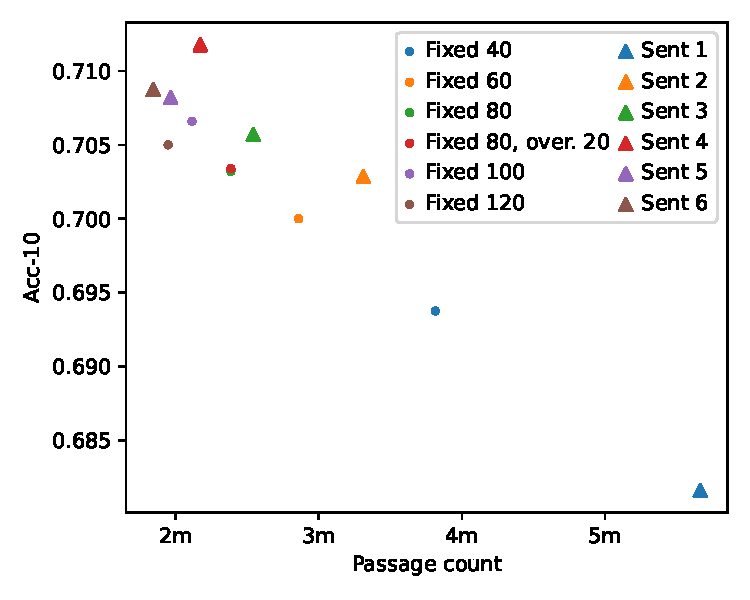
\includegraphics[width=0.7\linewidth]{img/split_intro.pdf}
    
    \caption{Retrieval performance and knowledge base size after being split using different methods. Note the cut-off y-axis.}
    \label{fig:split_intro}
\end{figure}

Surprisingly, the various splitting strategies are not vastly better than the default one (Fixed 100).
This can be attributed to using the DPR model, which is fine-tuned for retrieval and anything other than 100-token spans is outside of its finetuned input distribution.
An exception is that splitting on sentence boundaries (specifically Sent 5 and Sent 6) seems to be slightly systematically better than splitting at token count boundaries, even with the same number of passage counts.
This can be possibly explained via the examples introduced previously in this section.

\section{Filtering}

This section is concerned with reducing the knowledge-base size by simply filtering some of the spans which are deemed to not hold any interesting information and do not help with matching to the relevant document.
Either handcrafted or automatically derived, we are trying to find a function $h(d) \in \{0,1\}$ that classifies whether a given span should be retained and we construct a new set of spans as $\mathcal{S}' = \{d|d\in \mathcal{S} \wedge h(d)\}$.
For the following experiments, we use the splitting by 100 tokens so that the results are comparable across the thesis.
Again, we are interested in reducing the passage count while retaining the retrieval performance.

\subsection{Heuristics}

The most straightforward option is to remove spans that are too short, as shown in the introductory example.
\Cref{fig:filter_intro} shows the results with various filters based on either token or character count, i.e. $h_x(d) \Leftrightarrow \text{count}_\text{word/char}(d) \geq x$.
Unfortunately, any filtering measures show a strong regression against not using any filtering and thus this trade-off is not worth it.
Counterintuitively, this is true for also seemingly noninvasive heuristics, such as the number of words or characters being larger than 2 or 10, respectively.
The reason for this may be that these filtered short spans are not actual outliers, as shown by the distribution in \Cref{fig:filter_distribution}.

\begin{figure}[ht]
    \center
    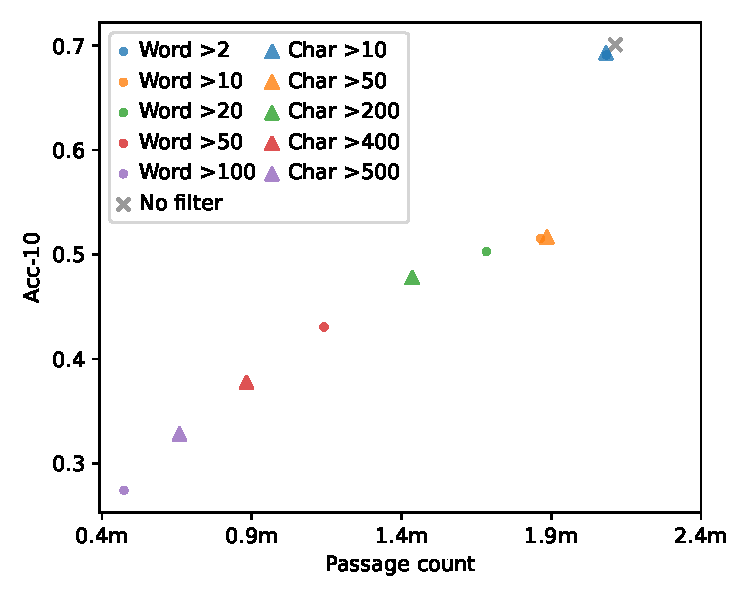
\includegraphics[width=0.7\linewidth]{img/filter_intro.pdf}
    
    \caption{Retrieval performance and knowledge base size after being filtered using length-based heuristics. Note the cut-off y-axis.}
    \label{fig:filter_intro}
\end{figure}


\begin{figure}[ht]
    \center
    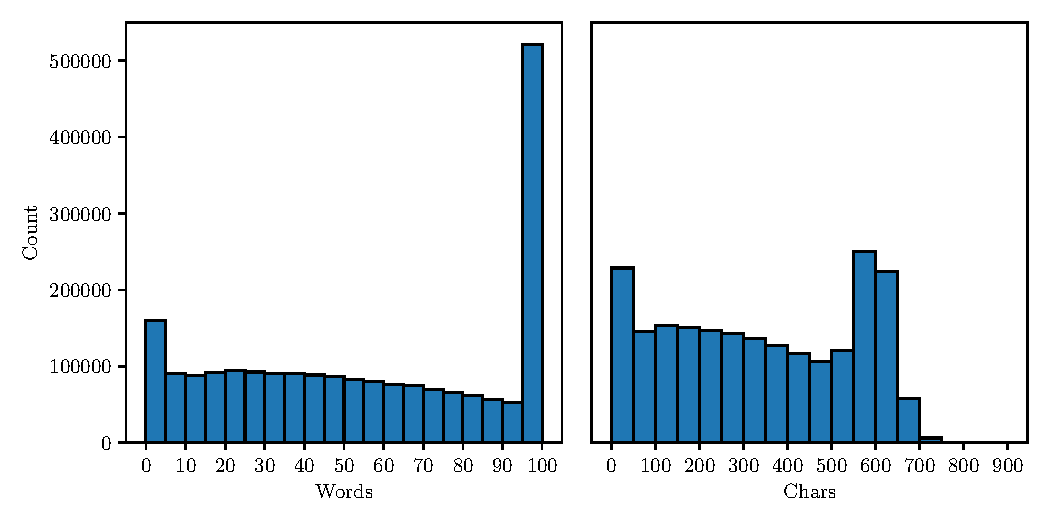
\includegraphics[width=\linewidth]{img/filter_distribution.pdf}
    
    \caption{Distribution of span length either with word or characte count.}
    \label{fig:filter_distribution}
\end{figure}

\subsection{Automatic filtering}

The issue with filtering using handcrafted heuristics is that it requires arbitrary human decision making and can not be automated.
Simple evaluation metrics, such as accuracy, consider top $k$ most similar spans to a query ($k$ is fixed).
The idea for automatic filtering is to simply remove span $s$ which satisfies the following two conditions given the training queries $Q_T$:
% TODO: math this?
\begin{itemize}
    \item \emph{At least one negative}: There exists at least one query for which this span is not relevant but for which it has been retrieved.
    \item \emph{Never positive}: No query for which this span is relevant retrieves it.
\end{itemize}

This filtering can be applied iteratively and two steps are visualized in \Cref{fig:autofilter}.
This algorithm is also described in pseudocode in \Cref{lst:autofilter}.

\begin{figure}[ht]
    \center
    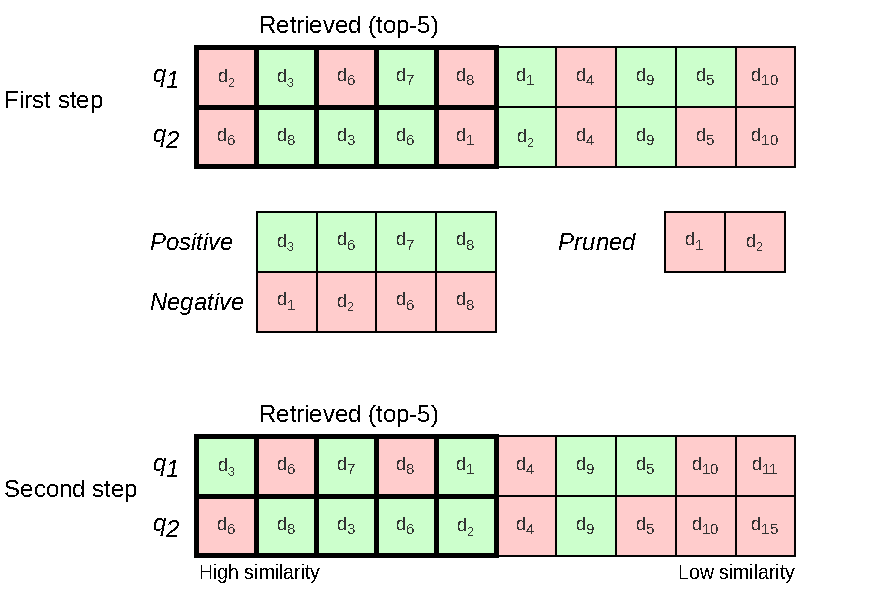
\includegraphics[width=0.95\linewidth]{img/autofilter.pdf}
    
    \caption{Example of two retrieval and one pruning steps on two queries. For both queries, the spans are sorted from left to right by decreasing similarity. Spans with bold borders are those considered as retrieved. Spans in green are relevant for the given query and spans in red are not relevant.}
    \label{fig:autofilter}
\end{figure}

\begin{minipage}{\linewidth}
    \begin{align*}
        & \textsc{FilterStep}(D, Q, k): \qquad\qquad\qquad\qquad\qquad \textit{spans and queries} \qquad\\
        & \qquad \text{Negative} \leftarrow \{\} \\
        & \qquad \text{Positive} \leftarrow \{\} \\
        & \qquad \textsc{For} \,\, (q_i, r_i) \in Q: \qquad\qquad\qquad\qquad\qquad \hspace{0.12cm}\textit{query and relevant spans} \\
        & \qquad \qquad d \leftarrow \textsc{Retrieve}_k(q_i) \\
        & \qquad \qquad \text{Negative} \leftarrow \text{Negative} \cup (d \setminus r_i) \\
        & \qquad \qquad \text{Positive} \leftarrow \text{Positive} \cup (d \cap r_i) \\
        & \qquad \text{Negative} \leftarrow  \text{Negative} \setminus \text{Positive} \\
        & \qquad D' \leftarrow D \setminus \text{Negative}
        \qquad\qquad\qquad\qquad\qquad \textit{prune spans} \\
        & \qquad \textit{out} \leftarrow (D', \text{Positive}, \text{Negative})
    \end{align*}
    \vspace{-0.8cm}
    \captionsetup{type=lstlisting}\caption{Definition of a single filtering step that prunes the spans and provides negative and positive samples}
    \label{lst:autofilter}
\end{minipage}

\clearpage

It is clear that by repeated application of this filtering step, the training retrieval performance is monotonous non-decreasing because we are never filtering spans that contribute positively to the metric.
Training accuracy is shown in the left of \Cref{fig:autofilter_dev_dev}.
The $k_f$ by which the top-$k_f$ spans in the filtering are considered can be the same as the $k_a$ in the accuracy evaluation metric.
If it is smaller than $k_a$, then the monotonicity property on the training data may not hold.
If it is larger, then we may get faster convergence, as shown on the right of \Cref{fig:autofilter_dev_dev}.
This is because we consider more negative and positive spans overall.

\begin{figure}[ht]
    \center
    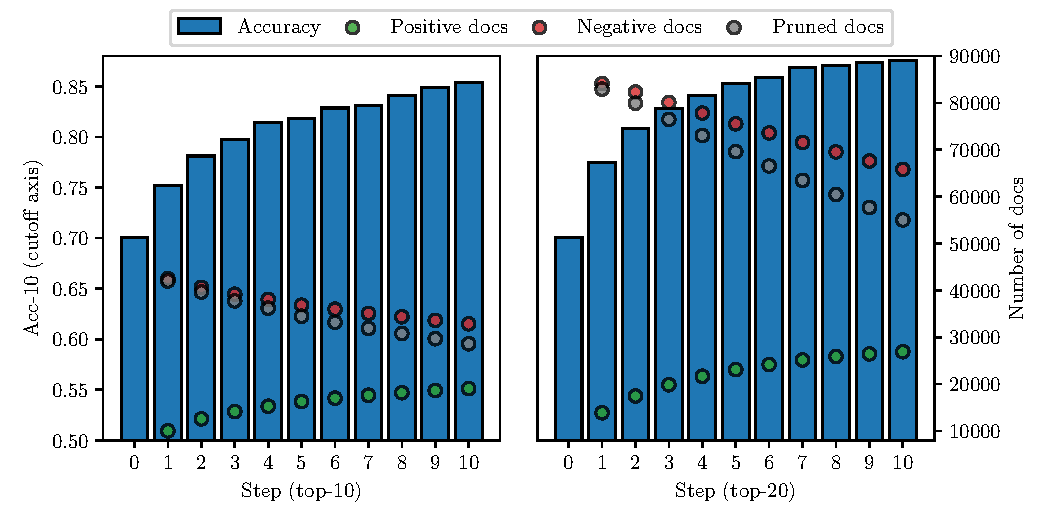
\includegraphics[width=\linewidth]{img/autofilter_dev_dev.pdf}
    \caption{Autofiltering performance of dev queries on spans filtered using the same dev queries. Filtering is done using either top-10 or top-20 spans.}
    \label{fig:autofilter_dev_dev}
\end{figure}

We are however interested in the performance on queries not seen during training.
There are two approaches that we consider: (1) using pruning based on training queries and (2) training a classifier to predict whether span is positive or only negative.
The results for the first one are shown in \Cref{fig:autofilter_train_dev} and unfortunately, the performance only deteriorates.
This is because even though the training and dev queries are drawn from the same distribution, this method has no way of generalizing and filtering only spans that are never relevant to any query (i.e. spans without any factual knowledge).

\begin{figure}[ht]
    \center
    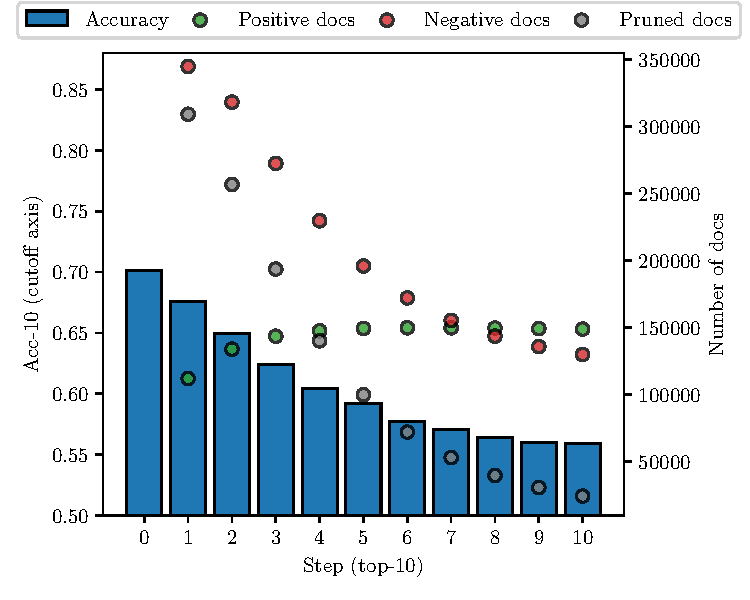
\includegraphics[width=0.8\linewidth]{img/autofilter_train_dev.pdf}
    \caption{Autofiltering performance of dev queries on spans filtered using train queries. Filtering is done using top-10 spans.}
    \label{fig:autofilter_train_dev}
\end{figure}


\begin{figure}[ht]
    \center
    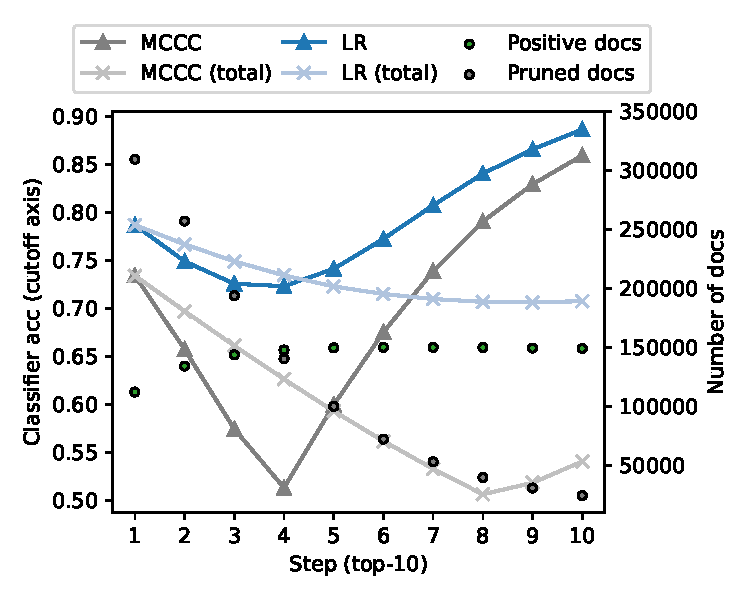
\includegraphics[width=0.8\linewidth]{img/autofilter_classifier.pdf}
    \caption{Training classifier accuracy for most common class classifier and logistic regression based on data from individual filtering steps or cummulative data up to a certain step (total).}
    \label{fig:autofilter_classifier}
\end{figure}

The other approach, which uses logistic regression to determine whether a span should be pruned, does not work either and by removing $\sim$5\% of spans regresses to 56\% retrieval accuracy in the first step.
Its performance is only marginally better than the most common class classifier, as shown in \Cref{fig:autofilter_classifier}.

\clearpage

\subsection{Discussion}

Neither manual based on span length nor automatic filtering showed any applicable results.
Manual filtering could be further enhanced with named entity recognition and allow only spans with e.g. at least one entity.

For automatic filtering, we would like to point out that we manipulated only positive and negative sets of spans and disregarded spans that were never retrieved.
Focusing on those is a venue for future work and could reduce the knowledge base size without affecting the retrieval performance neither positively nor negatively.
A possible solution to filter irretrievable spans is to consider spans that are least similar to the training queries, possibly via outlier detection methods.
Finally, we considered this filtering mechanism only on the level of vectors but it would be possible to also use the textual form of the span as well.